\documentclass[epsfig,a4paper,11pt,titlepage,oneside,openany]{book}
\usepackage{epsfig}
\usepackage{plain}
\usepackage{setspace}
\usepackage[paperheight=29.7cm,paperwidth=21cm,outer=2cm,inner=2cm,top=2cm,bottom=2cm]{geometry} % per definizione layout
\usepackage{titlesec} % per formato custom dei titoli dei capitoli
\usepackage{longtable}

%\usepackage[latin1]{inputenc} % per Windows;
\usepackage[utf8x]{inputenc} % per Linux (richiede il pacchetto unicode);
%\usepackage[applemac]{inputenc} % per Mac.

\singlespacing
\usepackage[english]{babel}

\usepackage{subfigure}
\usepackage{float}
\usepackage[table]{xcolor}
\usepackage{comment}
\usepackage{caption}
\usepackage{multirow}
\usepackage{wrapfig}
\usepackage{caption}
\usepackage{booktabs}


\begin{document}
	
	%\title{Research Project: Multimedia Data Security \\ Classification of sharing Applications}
	%\author{Kristjan Gjika}
	%\maketitle
	
	\pagenumbering{gobble} 
	\pagestyle{plain}
\thispagestyle{empty}

\begin{center}
	\begin{figure}[h!]
		\centerline{
\psfig{file=logo_unitn_black_center.eps,width=0.6\textwidth}}
	\end{figure}
	
	\vspace{2 cm} 
	
	\LARGE{Department of Engineering and Information Science\\}
	
	\vspace{1 cm} 
	\Large{Master in Computer Science\\}
	
	\vspace{2 cm} 
	\Large\textsc{Research Project in Multimedia Data Security\\} 
	\vspace{1 cm} 
	%\Huge\textsc{CONCISE SERVER-WIDE CAUSALITY MANAGEMENT FOR EVENTUALLY CONSISTENT DATA STORES \\}
	\Huge\textsc{Classification of Sharing Applications \\}
	\vspace{1 cm} 
	\Large{\today\\}
	\vspace{1 cm} 
	\vspace{1 cm} 
	%\Large{Giulia Zanella - 195385\\}
	%\Large{Kristjan Gjika - 196337\\}
	\begin{tabular*}{\textwidth}{ c @{\extracolsep{\fill}} c }
		\Large{Supervisors:} & \Large{Student:}\\
		\Large{Prof. Giulia Boato}& \Large{Kritjan Gjika}\\
		\Large{PHD. Quoc Tin Phan}& \\
	\end{tabular*}
	
	
	\vspace{1 cm} 
	
	\vspace{2 cm} 
	
	\Large{Academic Year 2018/2019}
	
\end{center}
	
	\clearpage
	
	\pagestyle{plain}
	
	\mainmatter
	
	\tableofcontents
	\clearpage
	
	
	\begingroup
	% nessuna interruzione di pagina tra capitoli
	% ridefinizione dei comandi di clear page
	\renewcommand{\cleardoublepage}{} 
	\renewcommand{\clearpage}{} 
	
	\titleformat{\chapter}
	{\normalfont\Huge\bfseries}{\thechapter}{1em}{}
	
	\titlespacing*{\chapter}{0pt}{0.59in}{0.02in}
	\titlespacing*{\section}{0pt}{0.20in}{0.02in}
	\titlespacing*{\subsection}{0pt}{0.10in}{0.02in}
	
%	\input{introduction}
%	\input{analisy}
%	\input{features}
	\chapter{Single Scenario Classification, KFold Validation}Starting with fitting randomly the classifiers, there are some statistics of the data used for the first test: \\
 {\def\arraystretch{1.3} 
 \begin{table}[H] 
\centering 
\begin{tabular}{|l|l|l|} 
\hline 
  &count train  &count test  \\ \hline
messenger  &249  &100  \\ \hline
telegram  &244  &106  \\ \hline
whatsapp  &243  &107  \\ \hline
original  &243  &107  \\ \hline
\end{tabular} 
\end{table} }
\section{Logistic regression results:} 
Confusion matrix with number of sample and with normalization:
 {\def\arraystretch{1.3} 
 \begin{table}[H] 
\centering 
\begin{tabular}{|l|l|l|l|l|} 
\hline 
  &messenger  &telegram  &whatsapp  &original  \\ \hline
messenger  &100  &0  &0  &0  \\ \hline
telegram  &0  &106  &0  &0  \\ \hline
whatsapp  &0  &0  &103  &4  \\ \hline
original  &0  &0  &0  &107  \\ \hline
\end{tabular} 
\end{table} }

 \begin{figure}[H] 
\centering 
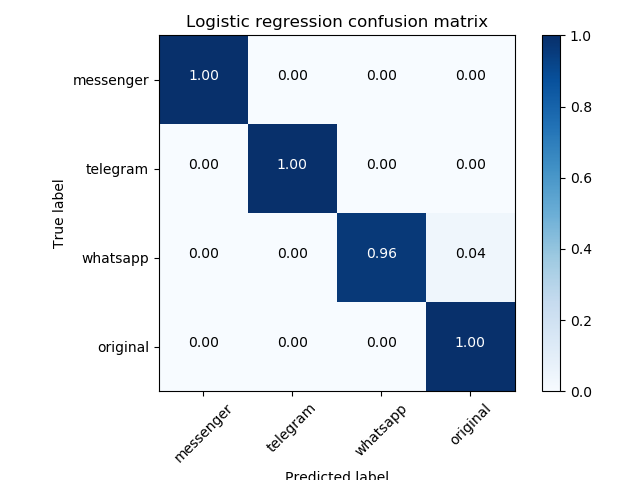
\includegraphics[scale=.6]{images/lr_initial.png} 
\caption{logistic regression} 
\end{figure} 


Result of the KFold validation with 10 bins:
 {\def\arraystretch{1.3} 
 \begin{table}[H] 
\centering 
\begin{tabular}{|l |l |l |l |l |l |l |l |l |l |}  
\hline 
1.0000&
0.9898&
0.9898&
1.0000&
1.0000&
0.9796&
0.9898&
1.0000&
0.9898&
1.0000\\ \hline  

\end{tabular} 
\end{table} }

The mean is : 0.993878\section{Linear Support Vector Machine results:}Confusion matrix with number of sample and with normalization:
 {\def\arraystretch{1.3} 
 \begin{table}[H] 
\centering 
\begin{tabular}{|l|l|l|l|l|} 
\hline 
  &messenger  &telegram  &whatsapp  &original  \\ \hline
messenger  &100  &0  &0  &0  \\ \hline
telegram  &0  &106  &0  &0  \\ \hline
whatsapp  &0  &0  &103  &4  \\ \hline
original  &0  &0  &0  &107  \\ \hline
\end{tabular} 
\end{table} }

 \begin{figure}[H] 
\centering 
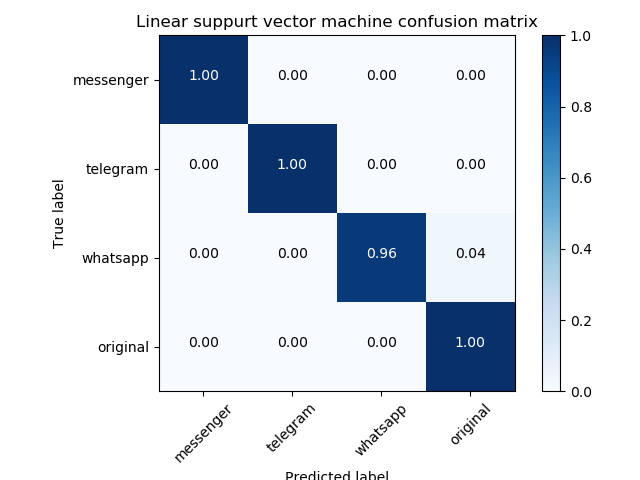
\includegraphics[scale=.6]{images/lsvm_initial.png} 
\caption{linear SVM} 
\end{figure} 


Result of the KFold validation with 10 bins:
 {\def\arraystretch{1.3} 
 \begin{table}[H] 
\centering 
\begin{tabular}{|l |l |l |l |l |l |l |l |l |l |}  
\hline 
1.0000&
0.9898&
1.0000&
1.0000&
1.0000&
0.9898&
0.9898&
1.0000&
0.9898&
1.0000\\ \hline  

\end{tabular} 
\end{table} }

The mean is : 0.995918\section{Random forest results:}Confusion matrix with number of sample and with normalization:
 {\def\arraystretch{1.3} 
 \begin{table}[H] 
\centering 
\begin{tabular}{|l|l|l|l|l|} 
\hline 
  &messenger  &telegram  &whatsapp  &original  \\ \hline
messenger  &100  &0  &0  &0  \\ \hline
telegram  &0  &106  &0  &0  \\ \hline
whatsapp  &0  &0  &103  &4  \\ \hline
original  &0  &0  &0  &107  \\ \hline
\end{tabular} 
\end{table} }

 \begin{figure}[H] 
\centering 
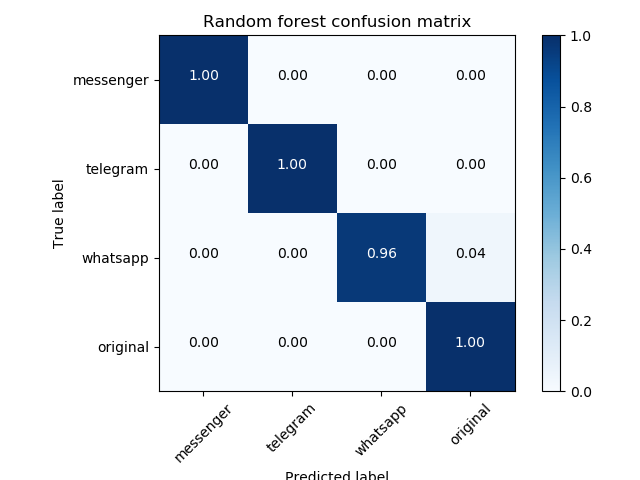
\includegraphics[scale=.6]{images/rf_initial.png} 
\caption{random forest} 
\end{figure} 


Result of the KFold validation with 10 bins:
 {\def\arraystretch{1.3} 
 \begin{table}[H] 
\centering 
\begin{tabular}{|l |l |l |l |l |l |l |l |l |l |}  
\hline 
0.9898&
0.9898&
1.0000&
1.0000&
1.0000&
0.9796&
0.9898&
1.0000&
0.9898&
1.0000\\ \hline  

\end{tabular} 
\end{table} }

The mean is : 0.993878

\chapter{Single Scenario Classification, Circularly Validation}

Here was used the same dataset as before but the training used a 0.3 of the dataset, and it is shifted circulary to cover all the dataset.Here is the table of all steps calculated \\
\begin{longtable} 
{|l |l |l |l |} 
\hline 
step  &logistic  &linear SVM  &random fo.  \\ \hline
0  &0.9831894364316239  &0.9791077839737224  &0.9870578936968979  \\ \hline
1  &0.9853026547006402  &0.9783844889010689  &0.9870578936968979  \\ \hline
2  &0.9853026547006402  &0.9775285159568015  &0.9909805452235539  \\ \hline
3  &0.9853026547006402  &0.9783844889010689  &0.9890580733784273  \\ \hline
4  &0.9871718848829855  &0.9783844889010689  &0.9890580733784273  \\ \hline
5  &0.981755684822845  &0.9908606639439437  &0.989920141798295  \\ \hline
6  &0.981755684822845  &0.9908606639439437  &0.989920141798295  \\ \hline
7  &0.981755684822845  &0.9908606639439437  &0.9888995950885928  \\ \hline
8  &0.981755684822845  &0.9908606639439437  &0.989920141798295  \\ \hline
9  &0.9797774593441748  &0.9846882267380576  &0.9836765977536278  \\ \hline
10  &0.9807773613945863  &0.9857299945019243  &0.9826969666799417  \\ \hline
11  &0.9807773613945863  &0.9846882267380576  &0.9826969666799417  \\ \hline
12  &0.9817853927299603  &0.9846882267380576  &0.9837044820834663  \\ \hline
13  &0.9817853927299603  &0.9857299945019243  &0.980725773647614  \\ \hline
14  &0.9817853927299603  &0.9857299945019243  &0.9817251354156551  \\ \hline
15  &0.9828271604938271  &0.9857299945019243  &0.9827641540487163  \\ \hline
16  &0.9828271604938271  &0.9857299945019243  &0.9827877082098887  \\ \hline
17  &0.9809303350970018  &0.9809303350970018  &0.9799310434556336  \\ \hline
18  &0.9809303350970018  &0.9809303350970018  &0.9799310434556336  \\ \hline
19  &0.9809303350970018  &0.9809303350970018  &0.9769817171132961  \\ \hline
20  &0.9809303350970018  &0.9809303350970018  &0.9799310434556336  \\ \hline
21  &0.9809303350970018  &0.9809303350970018  &0.9769817171132961  \\ \hline
22  &0.9779061415486145  &0.9799140749344002  &0.97795683313976  \\ \hline
23  &0.9779061415486145  &0.978906043599026  &0.9744170161392807  \\ \hline
24  &0.9779061415486145  &0.978906043599026  &0.9713928225908935  \\ \hline
25  &0.9779061415486145  &0.9779067519576579  &0.9769817171132961  \\ \hline
26  &0.9769068499072464  &0.9779067519576579  &0.9713928225908935  \\ \hline
27  &0.9820489340633134  &0.9849476193424314  &0.9820489340633134  \\ \hline
28  &0.9820489340633134  &0.9849476193424314  &0.9832038974293551  \\ \hline
29  &0.9820489340633134  &0.9808709993428069  &0.9801797038809681  \\ \hline
30  &0.9820489340633134  &0.9799805623885003  &0.9850731276117004  \\ \hline
31  &0.9820489340633134  &0.9799805623885003  &0.9850731276117004  \\ \hline
32  &0.9810570633546724  &0.9799144970334153  &0.9729849311036389  \\ \hline
33  &0.9627812747783722  &0.9583378598311828  &0.9542004398105941  \\ \hline
34  &0.953283825521887  &0.9489212587825018  &0.953283825521887  \\ \hline
35  &0.953283825521887  &0.9521822193250765  &0.9332107165025093  \\ \hline
36  &0.9521336702615147  &0.9510715431596557  &0.9342712270274949  \\ \hline
37  &0.9553966439474894  &0.9586655168859602  &0.941807112194959  \\ \hline
38  &0.9550624888401142  &0.9501411675781424  &0.941807112194959  \\ \hline
39  &0.9508728056918877  &0.957897835375157  &0.9435515300577979  \\ \hline
40  &0.949001628304907  &0.9569165446997437  &0.9426760297719203  \\ \hline
41  &0.949001628304907  &0.9570023590744005  &0.9426760297719203  \\ \hline
42  &0.9518168607439983  &0.9570023590744005  &0.9426760297719203  \\ \hline
43  &0.9628462719278571  &0.9690702601489536  &0.9670237271116444  \\ \hline
44  &0.9641308448001574  &0.9690415311211439  &0.9735226067675696  \\ \hline
45  &0.9611971340022054  &0.9540513512651186  &0.9735226067675696  \\ \hline
46  &0.9636358185061074  &0.9539595767948307  &0.9691897607151013  \\ \hline
47  &0.9634237045681469  &0.9549009600982763  &0.9713033424446343  \\ \hline
48  &0.9630416021422119  &0.9457796737082027  &0.9724089271961905  \\ \hline
49  &0.9590950950950952  &0.9645468263150108  &0.9631028529724224  \\ \hline
50  &0.9590950950950952  &0.9645468263150108  &0.9651904231493449  \\ \hline
51  &0.9590950950950952  &0.9645468263150108  &0.9651904231493449  \\ \hline
52  &0.9590950950950952  &0.9645468263150108  &0.9651904231493449  \\ \hline
53  &0.9704082737708469  &0.9750147841513898  &0.9745533102297715  \\ \hline
54  &0.9749984999849999  &0.9794007490636705  &0.9800443458980044  \\ \hline
55  &0.9749984999849999  &0.9794007490636705  &0.9778754788737738  \\ \hline
56  &0.9749984999849999  &0.9794007490636705  &0.9789560728306903  \\ \hline
57  &0.9765285344002652  &0.9802631578947368  &0.9790280857354028  \\ \hline
58  &0.9775769230769231  &0.9802631578947368  &0.9779480414953162  \\ \hline
59  &0.9775769230769231  &0.9802631578947368  &0.9791724190826814  \\ \hline
60  &0.9756841360427018  &0.978544776119403  &0.9780137313157126  \\ \hline
61  &0.9757692307692307  &0.978544776119403  &0.9780893448656607  \\ \hline
62  &0.9746787205323791  &0.9794007490636705  &0.980188679245283  \\ \hline
63  &0.9959839357429718  &0.9989837398373984  &0.9989837398373984  \\ \hline
64  &0.9899551291586098  &0.9949676755803702  &0.9898723422423363  \\ \hline
65  &0.9814065924422243  &0.989179818268771  &0.9850946868966615  \\ \hline
66  &0.9851206921404461  &0.989179818268771  &0.9881081682594579  \\ \hline
67  &0.983242407923623  &0.9801158153090965  &0.9831320060410063  \\ \hline
68  &0.9841779184557378  &0.9791077839737224  &0.9900154191754695  \\ \hline
69  &0.9841779184557378  &0.9791077839737224  &0.987165432614862  \\ \hline
\end{longtable} 
Average of all steps: 

 {\def\arraystretch{1.3} 
 \begin{table}[H] 
\centering 
\begin{tabular}{|l|l|l|} 
\hline 
logistic r.  &linear SVM  &random f.  \\ \hline
0.9742098967923488  &0.9754435548603985  &0.9748451176133341  \\ \hline
\end{tabular} 
\end{table} }
Confusion matrix estimated on overall tests: 

 \begin{figure}[H] 
\centering 
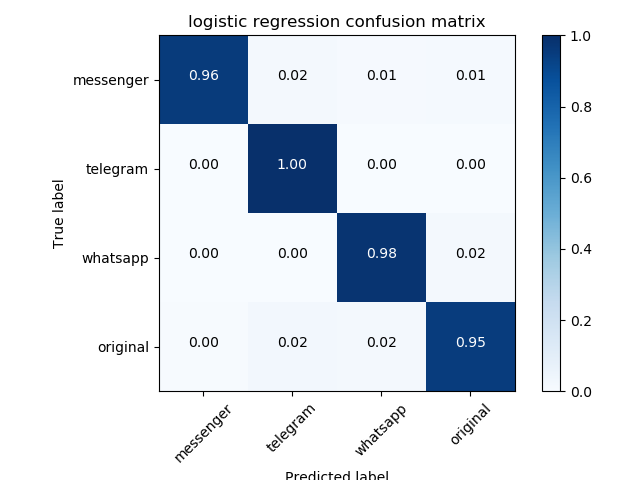
\includegraphics[scale=.6]{images/logistic_total.png} 
\caption{logistic regression} 
\end{figure} 

 \begin{figure}[H] 
\centering 
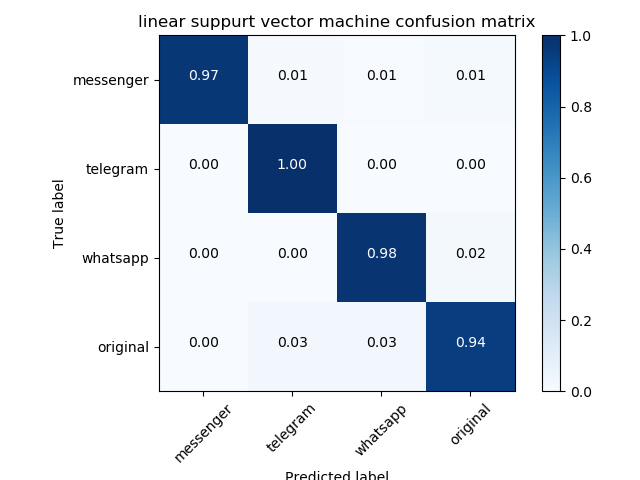
\includegraphics[scale=.6]{images/lsvm_total.png} 
\caption{linear SVM} 
\end{figure} 

 \begin{figure}[H] 
\centering 
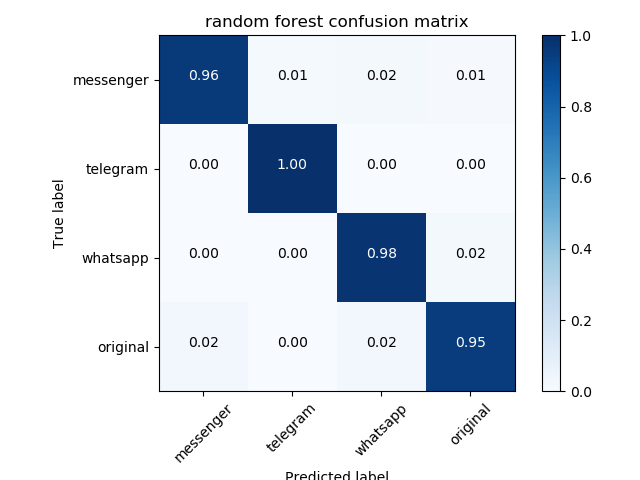
\includegraphics[scale=.6]{images/random_total.png} 
\caption{random forest} 
\end{figure} 

	%\input{report_double}
	%\input{flow}
%	\input{report_double_parte1.tex}
%	\input{report_double_parte2.tex}
%	\input{report_double_parte3.tex}
%	\input{new_methods.tex}
%	\input{conclusions.tex}
	%\input{report_double_parte4_.tex}
		
	\endgroup
	
	\addcontentsline{toc}{chapter}{Bibliografia}
	% stile con ordinamento alfabetico in funzione degli autori
	\bibliographystyle{plain}
	\bibliography{biblio}
	%\cellcolor{blue!25}
	
\end{document}